\documentclass[usenames,dvipsnames]{beamer}

\usetheme[bgphoto]{polimi}
% \usetheme{Madrid}
\usepackage[utf8]{inputenc}
\usepackage{appendixnumberbeamer}
\usepackage{array,multirow,booktabs}
\usepackage{lipsum}
\usepackage[font=scriptsize]{caption}
\usepackage{microtype}
\usepackage{subfig}
\usepackage[hyphens]{xurl}
\usepackage{hyperref}
\usepackage{amsmath,amssymb}
\DeclareMathSymbol{\mlq}{\mathrel}{operators}{``}
\DeclareMathSymbol{\mrq}{\mathrel}{operators}{`'}
\setbeamertemplate{frametitle continuation}{}

\usepackage[natbib=true,citestyle=authoryear,bibstyle=numeric,backend=bibtex]{biblatex}
\setlength\bibitemsep{1.5\itemsep}
\renewcommand*{\nameyeardelim}{\addcomma\space}
\renewcommand*{\bibfont}{\footnotesize}
%\setbeamertemplate{bibliography item}{}
\defbibenvironment{bibliography}
  {\list
     {}
     {\setlength{\leftmargin}{\bibhang}%
      \setlength{\itemindent}{-\leftmargin}%
      \setlength{\itemsep}{\bibitemsep}%
      \setlength{\parsep}{\bibparsep}}}
  {\endlist}
  {\item}
\addbibresource{references.bib}

% Full instructions available at:
% https://github.com/elauksap/beamerthemepolimi

\title{Gender Discrimination in Data Analysis:\\a Socio-Technical Approach}
\author{Riccardo Corona}
\date{07/10/2021}


\begin{document}
    \begin{frame}
        \maketitle
    \end{frame}
    
    
    \begin{frame}{Research Context}
        \begin{block}{Data analysis}
            Set of processes for inspecting, cleaning, transforming, and modeling data with the aim of discovering useful information, informing conclusions, and supporting decision making.
        \end{block}
        \begin{block}{Gender discrimination}
            Specific (sub)category of social problems, here expressed in the form of the so-called `\textbf{gender gap}', definable as:
            \begin{quote}
            \emph{A difference between the way men and women are treated in society, or between what men and women do and achieve.} \parencite{cambridge2013gender}
            \end{quote}
        \end{block}
    \end{frame}
    
    
    \begin{frame}{Scenarios \& Problem Statement}
        \begin{block}{Problem}
            Data and datasets, on which a lot of actions of our daily routine are based, can be \textbf {unfair}. Unfair, or better to say, \textbf{biased} data, may influence, directly or indirectly, our perception of reality, and lead us to make decisions that, although seemingly fair and just, contain in turn bias, and discriminate against individuals or groups of individuals.
        \end{block}
        \begin{exampleblock}{Example scenarios}
            \begin{itemize}
                \item \textcolor{greenPolimi}{COMPAS} tool used in the U.S. to predict recidivism risk biased against Black people. \emph{\parencite{angwin2016machine}}
                \item \textcolor{greenPolimi}{Amazon} software to screen candidates for employment biased against women. \emph{\parencite{dastin2018amazon}}
            \end{itemize}
        \end{exampleblock}
    \end{frame}
    
    
    \begin{frame}{Methodology}
        \textbf{Dual perspective} on the problem: qualitative and conceptual approach typical of sociology combined with technical and pragmatic approach of engineering and computer science.
        	\begin{itemize}
        	    \item Systematic literature review.
        	    \item Experimental case studies through Python and Jupyter Notebook to verify not only whether or not men and women are paid fairly, but also if there are other collateral issues related to gender discrimination in the data and what tools can possibly catch them.
        	    \item Technical results discussed in the light of the sociological background.
        	\end{itemize}
        	 We try to understand to what extent the problem is to be found in the \textit{instrumentation and technical choices} and to what extent it is instead rooted in \textit{society}.
    \end{frame}
    
    
    \begin{frame}{Sociological Perspective}
        \begin{block}{Global Gender Gap Index}
            Cumulative measure for ranking countries which benchmarks national gender gaps on economic, education, health, and political criteria.
        \end{block}
        U.S. ranking: 49/144, overall score: 0.718 (1 = gender parity)\newline $\rightarrow$ men more participatory in labor force; women tend to earn less than men, be employed part-time, or not to be paid for their work, and are underrepresented in managerial and higher-paying jobs.\newline\newline Some possible reasons:
        \begin{itemize}
            \item Statistical discrimination \emph{\parencite{tilcsik2021statistical}}
            \item Institutional environment \emph{\parencite{beggs1995institutional}}
            \item Unequal bargaining power \emph{\parencite{folbre2021gender}}
        \end{itemize}
    \end{frame}
    
    
    \begin{frame}{Sociological Perspective -- Data \& Statistics}
        \begin{figure}
            \subfloat{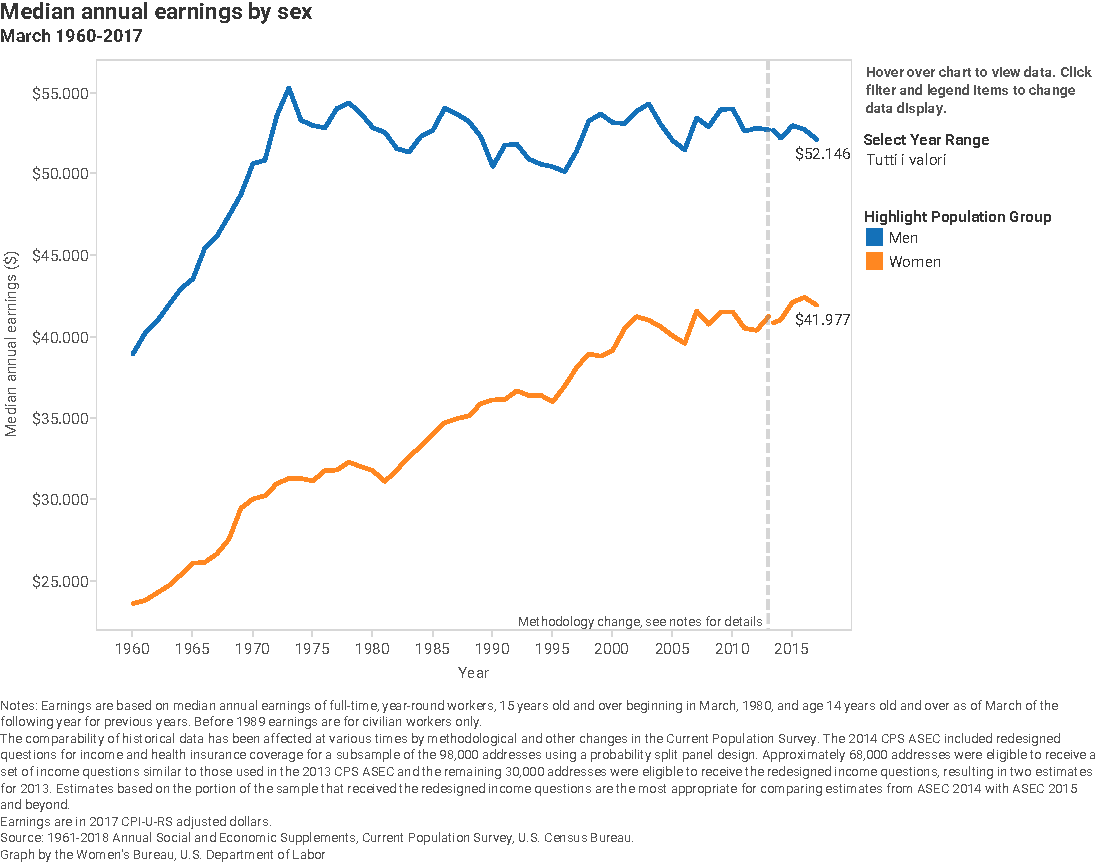
\includegraphics[width=0.475\textwidth]{figures/dol_earnings_by_sex.pdf}}
            \hfill
            \subfloat{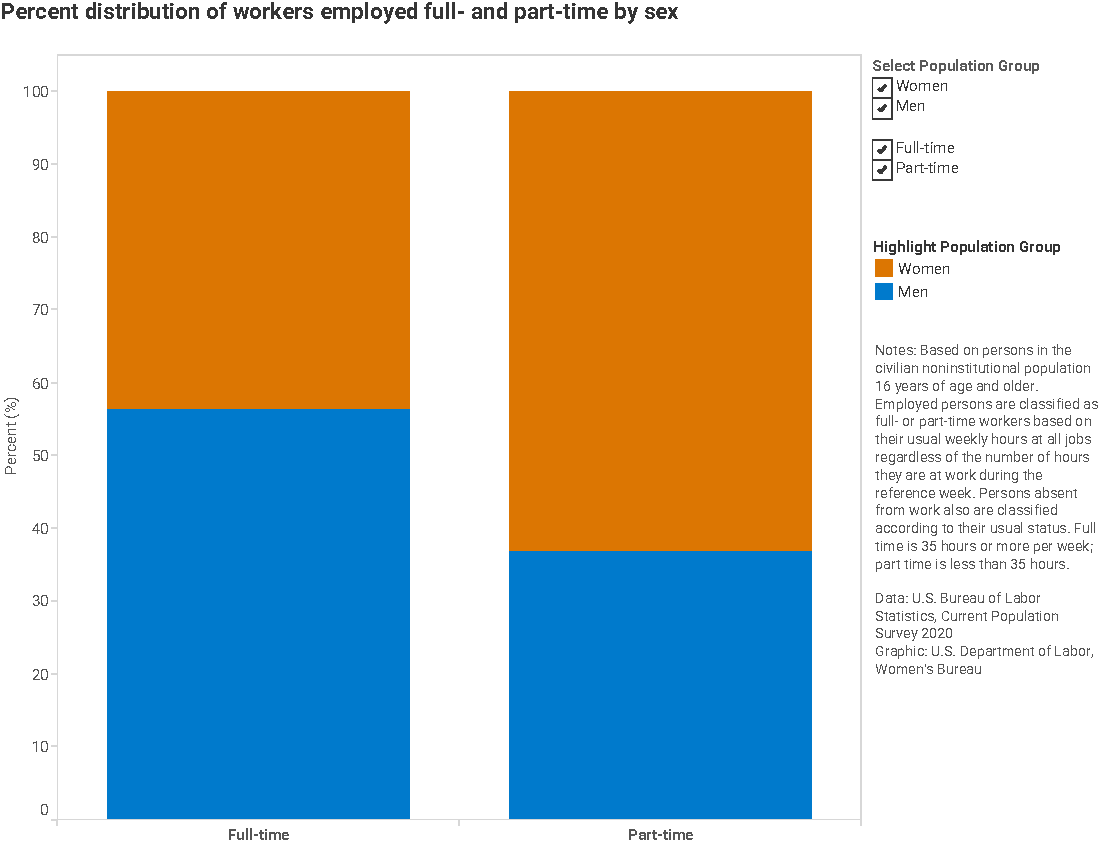
\includegraphics[width=0.475\textwidth]{figures/dol_full-_and_part-time_workers_by_sex.pdf}}
        \end{figure}
    \end{frame}
    
    
    \begin{frame}{Sociological Perspective -- Data \& Statistics}
        \begin{figure}
            \subfloat{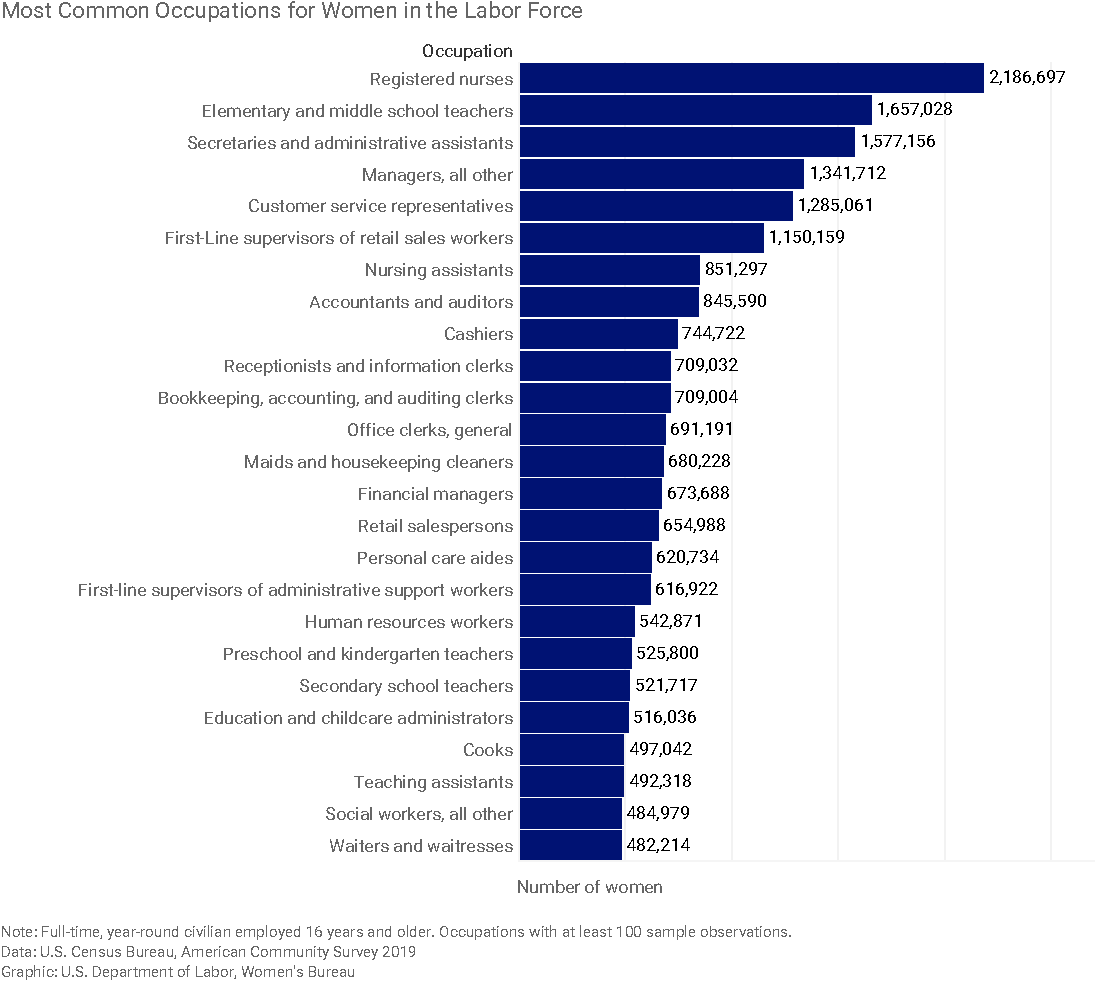
\includegraphics[width=0.475\textwidth]{figures/dol_most_common_occupations_women.pdf}}
            \hfill
            \subfloat{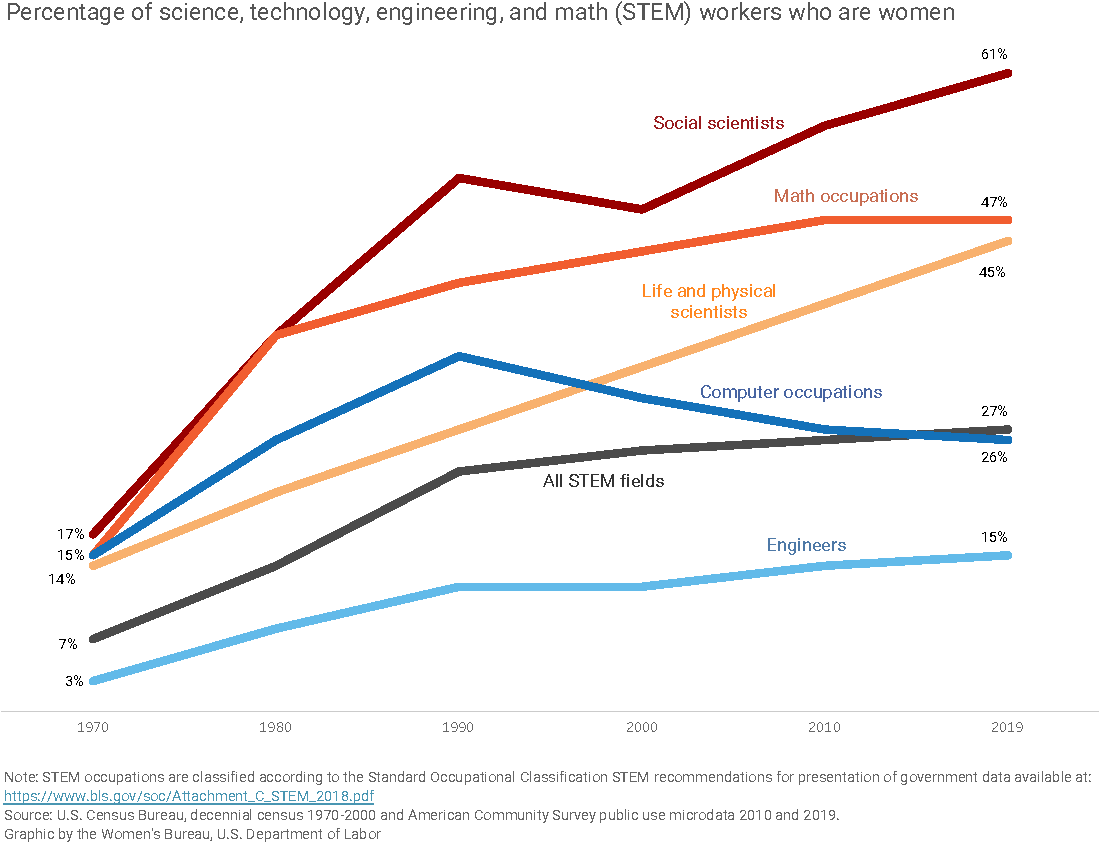
\includegraphics[width=0.475\textwidth]{figures/dol_stem_percent_women.pdf}}
        \end{figure}
    \end{frame}
    
    
    \begin{frame}{Tools for Assessing Fairness}
        \begin{itemize}
            \item \textit{The `Glassdoor Method'}: a framework for evaluating gender pay gap which relies on \textbf{linear regression}. \emph{\parencite{chamberlain2017analyze}}
        \end{itemize}
        \begin{block}{Linear regression}
            \begin{columns}
                \begin{column}{0.4715\textwidth}
                    Preprocessing technique used to smooth out noise or to find patterns within a dataset, which attempts to model the relationship between two or more variables by fitting data to a linear equation. \[y = \beta_0 + \beta_1x + \epsilon\]
                \end{column}
                \begin{column}{0.4715\textwidth}
                    \begin{center}
                        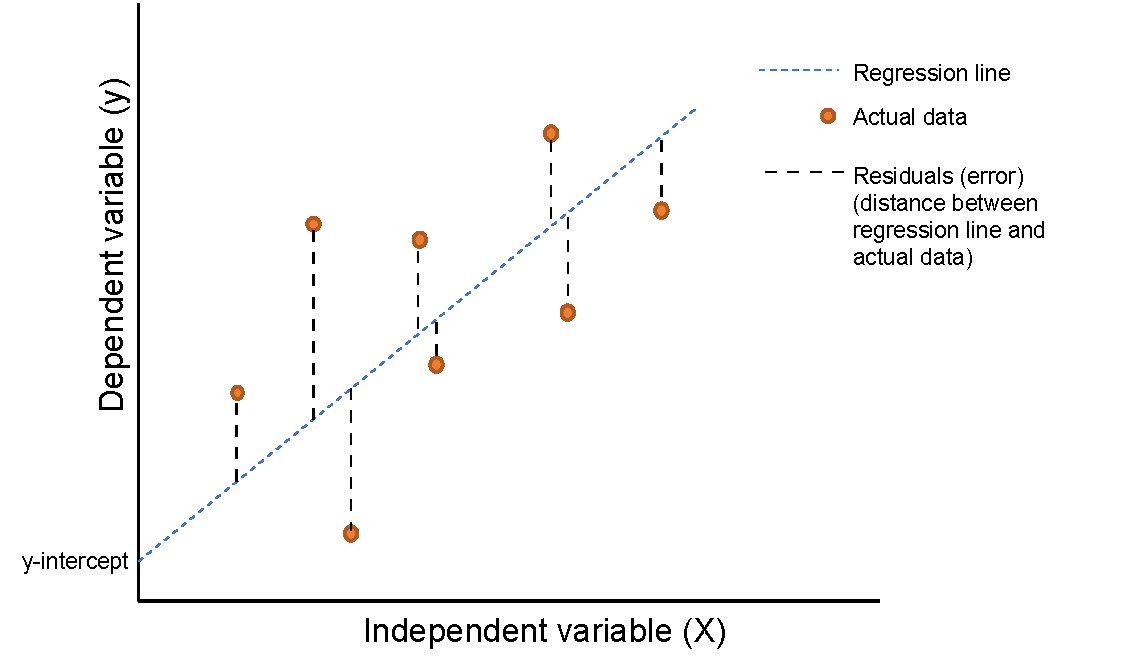
\includegraphics[width=\textwidth]{figures/simple_linear_regression.pdf}
                    \end{center}
                \end{column}
            \end{columns}
        \end{block}
    \end{frame}
    
    
    \begin{frame}{Tools for Assessing Fairness}
        \begin{itemize}
            \item \textit{FAIR-DB}: an algorithm to detect bias in data based on \textbf{functional dependencies} and the related evaluation metrics. \emph{\parencite{azzalini2021fair}}
        \end{itemize}
        \begin{block}{Functional Dependencies (FDs)}
            Constraint involving two (sets of) attributes of the same relation in which the first \textit{uniquely determines} the second.
        \end{block}
        \begin{block}{Approximate Conditional Functional Dependencies (ACFDs)}
            FDs holding on a subset of tuples (Approximate) which use conditions on attribute values to specify the subset on which they hold (Conditional).
            \[\mathit{Status} = \mlq \mathrm{F} \mrq, \mathit{Gender} = \mlq \mathrm{female} \mrq \rightarrow \mathit{Annual Salary Bin} = \mlq \leq \mathrm{90K} \mrq\]
        \end{block}
    \end{frame}
    
    
    \begin{frame}{Tools for Assessing Fairness}
        \begin{itemize}
            \item \textit{Ranking Facts}: an application built on the idea of \textbf{ranking} which makes use of three statistical measures to evaluate fairness. \emph{\parencite{yang2018nutritional}}
            \begin{itemize}
                \item \textbf{FA*IR}: compares the number of protected elements in every prefix of the ranking (i.e., the top-\(i\) positions, with \(i \in [1, k]\)) with the expected number of protected elements if they were picked at random using Bernoulli trials with success probability \(p\).
                \item \textbf{Proportion}: statistical measure based on the concept of \textit{(two sample) z-test} -- particular type of hypothesis test which allows to compare two proportions to check whether they are the same or not.
                \item \textbf{Pairwise}: compares options in pairs and determines which is the preferred choice or has the highest level of importance based on defined criteria. At the end of the comparison process, each option has a rank or relative rating as compared to the others.
            \end{itemize}
        \end{itemize}
    \end{frame}
    
    
    \begin{frame}{Case Study 1: Chicago}
        \begin{itemize}
            \item \textbf{Data preprocessing}: 20,309 tuples, of which 16,146 males and 4,163 females, and with 35 distinct \textit{Job Title} values and 20 distinct \textit{Department} values.\newline
            \item \textbf{The `Glassdoor Method'}: 24.2\% `unadjusted' pay gap; 0.4\% `adjusted' pay gap $\rightarrow$ no evidence of a systematic gender pay gap.
            \item \textbf{FAIR-DB}: 6 final functional dependencies; 11.4\% of the dataset `problematic' $\rightarrow$ dataset quite fair.
            \item \textbf{Ranking Facts}: dataset fair for both males and females, for each statistical measure.
        \end{itemize}
    \end{frame}
    
    
    \begin{frame}{Case Study 1: Chicago}
        \begin{figure}
            \subfloat{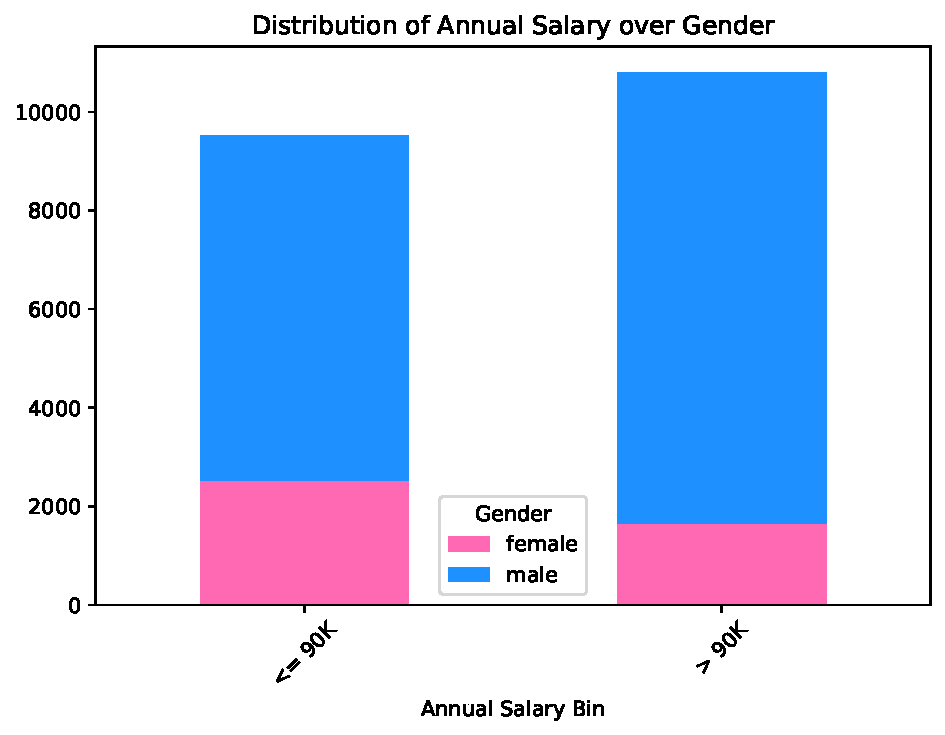
\includegraphics[width=0.475\textwidth]{figures/chicago_2bins_annual_salary_over_gender.pdf}}
            \hfill
            \subfloat{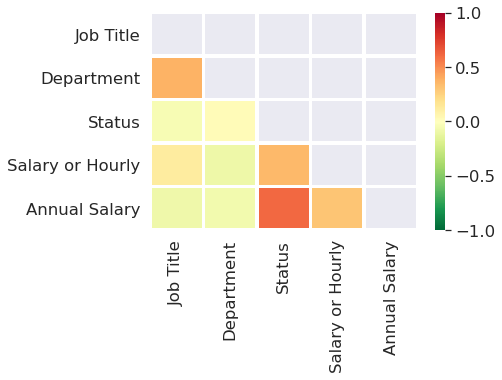
\includegraphics[width=0.475\textwidth]{figures/chicago_rankingfacts1.png}}
        \end{figure}
    \end{frame}
    
    
    \begin{frame}{Case Study 2: San Francisco}
        \begin{itemize}
            \item \textbf{Data preprocessing}: 22,996 tuples, of which 13,688 males and 9,308 females, and with 81 distinct \textit{Job Title} values.\newline
            \item \textbf{The `Glassdoor Method'}: 30.4\% `unadjusted' pay gap; \(-\)5\% `adjusted' pay gap $\rightarrow$ no evidence of a systematic gender pay gap.
            \item \textbf{FAIR-DB}: 10 final functional dependencies; 24.3\% of the dataset `problematic' $\rightarrow$ dataset quite fair because of the low values of \textit{difference} (`unfairness level') and \textit{support} (number of tuples involved), but for higher-paying jobs men seem to have an economic advantage over women.
            \item \textbf{Ranking Facts}: dataset fair for males and unfair for females, for each statistical measure $\rightarrow$ proportion of women in the top-\(k\) ranking effectively very low.
        \end{itemize}
    \end{frame}
    
    
    \begin{frame}{Case Study 2: San Francisco}
        \begin{figure}
            \subfloat{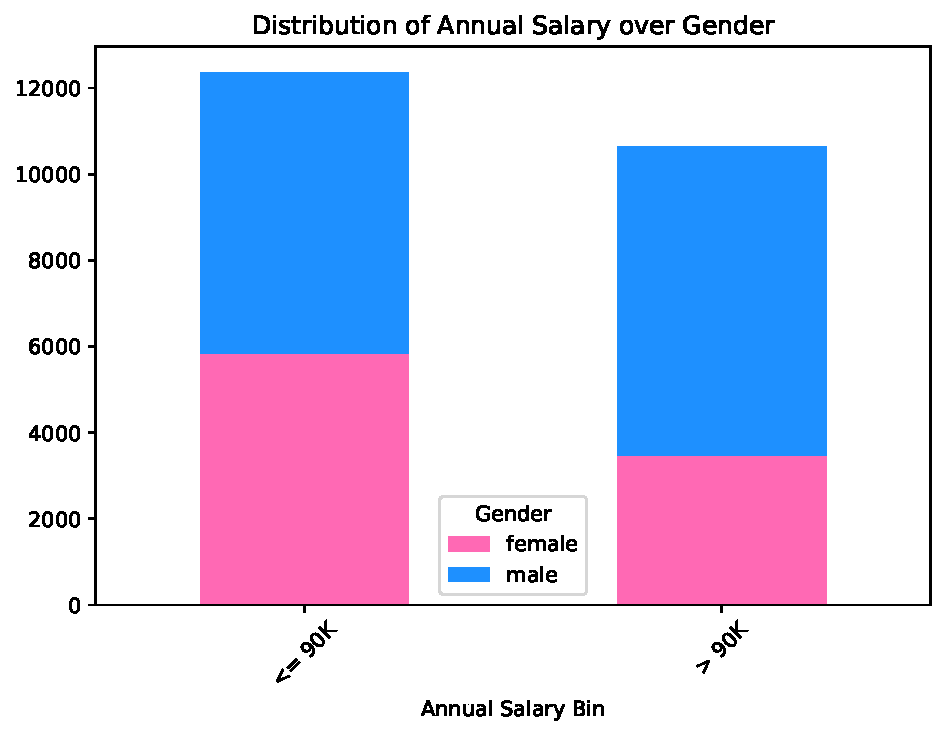
\includegraphics[width=0.475\textwidth]{figures/san_francisco_2bins_annual_salary_over_gender.pdf}}
            \hfill
            \subfloat{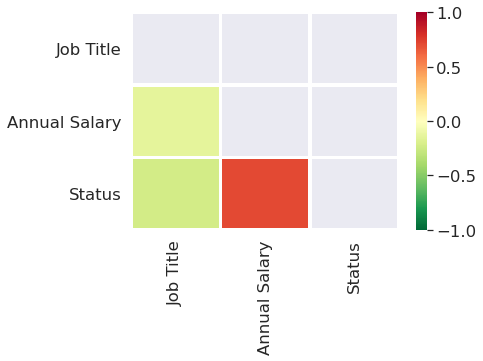
\includegraphics[width=0.475\textwidth]{figures/san_francisco_rankingfacts1.png}}
        \end{figure}
    \end{frame}
    
    
    \begin{frame}{Other Design Choices}
        \begin{itemize}
            \item \textbf{Part-time employees removal}: most of the tuples removed related to women (Chicago); excessive amount of tuples removed (San Francisco).
            \item \textbf{FAIR-DB: discretization using more bins}: less and different final dependencies detected (Chicago and San Francisco).
            \item \textbf{FAIR-DB: choice of different dependencies}: 85.6\% (Chicago) and 92.5\% (San Francisco) of the dataset `problematic'.
            \item \textbf{Grouping of job titles}: overturning of the outcomes for Ranking Facts (Chicago dataset unfair for males and fair for females, for each statistical measure).
            \item \textbf{Voluntary introduction of bias}: results from each tool oriented toward unfair Chicago dataset, in which women are discriminated against (retaining 50\%, 75\%, and 90\% of the \textit{Annual Salary} value of female employees).
        \end{itemize}
    \end{frame}
    
    
    \begin{frame}{Outcomes}
        \begin{itemize}
            \item Strengths and weaknesses of the tools highlight their non-exhaustiveness and complementarity.
            \item Tools practically fail in capturing the several facets of \textit{equity}.
            \begin{block}{Equity}
                The idea that people should have access to resources (possibly of a different nature and to a different extent) in order to be able to reach the same condition.
            \end{block}
            \item \textbf{Representation problem}: disproportion in the percentage of women employed in different sectors.
            \item \textbf{Part-time problem}: higher number of women employed in part-time jobs, typically less paid than full-time ones.
        \end{itemize}
    \end{frame}
    
    
    \begin{frame}{Contributions}
        \begin{itemize}
            \item Fairness is a multifaceted concept which cannot be exhausted by providing a single definition and pursuing that specific definition experimentally.
            \item Tools are susceptible to decisional choices, and therefore users must be properly trained on the specific area of analysis.
            \item Double perspective on the gender pay gap issue emphasized the importance of multidisciplinarity, especially when dealing with problems of an ethical and sociological nature.
        \end{itemize}
    \end{frame}
    
    
    \begin{frame}{(Some) Limitations}
        \begin{itemize}
            \item Sociological
            \begin{itemize}
                \item Non-specific literature
                \item No direct insights from U.S. workers
            \end{itemize}
            \item Technical
            \begin{itemize}
                \item Original datasets already partial or possibly grouped
                \item \texttt{gender-guesser} (package to infer employees' gender)
            \end{itemize}
            \item Design
            \begin{itemize}
                \item Removal of job titles with less than 100 occurrences
                \item FAIR-DB: parameter values; manual selection of rules; number of bins
            \end{itemize}
        \end{itemize}
    \end{frame}
    
    
    \begin{frame}{Future Work}
        \begin{itemize}
            \item Combine all the tools in a unique, more complete instrument, possibly trying to encompass even more facets of equity, or more definitions of fairness.
            \item Support analyses of this kind by sociological research.
            \item Enrich sociological research by conducting an interview with workers and HR practitioners of the cities under study.
            \item Retrieve further information in support of the mere data and create effective documentation, possibly pointing at \textbf{context-awareness} (provide the tools with knowledge on the context of use).
        \end{itemize}
    \end{frame}
    
    
    \begin{frame}
        \centering \huge Thank you!\\
        \vspace{\baselineskip}
        \centering \Large Any question?
    \end{frame}
    
    
    \begin{frame}[allowframebreaks]{References}
        \printbibliography
    \end{frame}
\end{document}
